\documentclass[sigconf]{acmart}

\usepackage{graphicx}
\usepackage{algorithm} % for algorithms
\usepackage{algpseudocode}
\usepackage{booktabs} % For formal tables
\usepackage{amsthm} % For claims
\usepackage{bbm} % indicator function

% table
\usepackage[flushleft]{threeparttable} % http://ctan.org/pkg/threeparttable
\usepackage{booktabs,caption}

\theoremstyle{remark}

\settopmatter{printacmref=true, printccs=true, printfolios=true}
\pagestyle{empty} % removes running headers

\newcommand{\PicScale}{0.5}
\newcommand {\FlameStream} {FlameStream}
\begin{document}

\copyrightyear{2019} 
\acmYear{2019} 
\acmConference[BIRTE 2019]{Real-Time Business Intelligence and Analytics}{August 26, 2019}{Los Angeles, CA, USA}
\acmBooktitle{Real-Time Business Intelligence and Analytics (BIRTE 2019), August 26, 2019, Los Angeles, CA, USA}
\acmPrice{15.00}
\acmDOI{10.1145/3350489.3350491}
\acmISBN{978-1-4503-7660-0/19/08}

\title {Distributed Classification of Text Streams: Limitations, Challenges, and Solutions}

% \author{Artem Trofimov,$^ {1}$   Nikita Sokolov,$^{2}$    Mikhail Shavkunov,$^3$   Igor E. Kuralenok,$^1$    and  Boris Novikov$^ {3}$ }
% \affiliation{%
% \institution{$^1$JetBrains Research}
% }
% \affiliation{%
% \institution{$^2$ ITMO University}
% }
% \affiliation{%
% \institution{$^3$National Research University Higher School of Economics}
% \city{St. Petersburg} 
% \country{Russia}
% }
% \email{\string{trofimov9artem, faucct, mv.shavkunov, ikuralenok\string}@gmail.com, borisnov@acm.org}

\author{Artem Trofimov}
\affiliation{%
  \institution{Saint Petersburg State University / Yandex}
  \city{Saint Petersburg}
  \country{Russia}}
\email{tomato@yandex-team.ru}

\author{Nikita Sokolov}
\affiliation{%
  \institution{ITMO university}
  \city{Saint Petersburg}
  \country{Russia}}
\email{faucct@gmail.com}

\author{Mikhail Shavkunov}
\affiliation{%
  \institution{National Research University Higher School of Economics}
  \city{Saint Petersburg}
  \country{Russia}}
\email{mv.shavkunov@gmail.com}

\author{Igor Kuralenok}
\affiliation{%
  \institution{Yandex}
  \city{Saint Petersburg}
  \country{Russia}}
\email{solar@yandex-team.ru}

\author{Boris Novikov}
\affiliation{%
  \institution{National Research University Higher School of Economics}
  \city{Saint Petersburg}
  \country{Russia}}
\email{borisnov@acm.org}

\begin{abstract}

Large-scale classification of text streams is an essential problem that is hard to solve. Batch processing systems are scalable and proved their effectiveness for this problem but do not provide low latency. On the other hand, state-of-the-art distributed stream processing systems are able to achieve low latency but do not support the same level of fault tolerance and determinism. In this work, we discuss how the distributed streaming computational model and fault tolerance mechanisms can affect the results of a typical text classification data flow. We demonstrate emerged trade-offs between fault tolerance and reproducibility on the one side, and performance on the other side. Potential ways to solve the revealed issues and to handle streaming features are proposed.

\end{abstract}

\begin{CCSXML}
\begin{CCSXML}
\begin{CCSXML}
<ccs2012>
<concept>
<concept_id>10002951.10002952.10002953.10010820.10003208</concept_id>
<concept_desc>Information systems~Data streams</concept_desc>
<concept_significance>500</concept_significance>
</concept>
<concept>
<concept_id>10002951.10003317.10003347.10003356</concept_id>
<concept_desc>Information systems~Clustering and classification</concept_desc>
<concept_significance>500</concept_significance>
</concept>
<concept>
<concept_id>10002951.10003227.10003351.10003446</concept_id>
<concept_desc>Information systems~Data stream mining</concept_desc>
<concept_significance>300</concept_significance>
</concept>
</ccs2012>
\end{CCSXML}

\ccsdesc[500]{Information systems~Data streams}
\ccsdesc[500]{Information systems~Clustering and classification}
\ccsdesc[300]{Information systems~Data stream mining}

\keywords{Data streams, text classification, reproducibility, exactly-once}

\maketitle

\thispagestyle{empty}

\section {Introduction}
\label {fs-short-intro}

Classification of large text streams is hard, but important task for researchers and practitioners. It has a wide range of applications including detection of emerging news and current user interests, suspicious traffic analysis, spam filtering, etc. Popular open-source libraries like sklearn~\cite{sklearn_api} and NLTK~\cite{bird2009natural} provide a rich set of tools, but they mostly aim at handling static datasets. The lack of scalability across multiple computational units is another limitation of these solutions. There are plenty of works which adapt batch processing systems for text classification~\cite{semberecki2016distributed, svyatkovskiy2016large, baltas2016apache}. Their advantages are fault tolerance, high throughput, and scalability. On the other hand, these systems do not provide low latency that is a strong requirement for most streaming applications.

An immediate idea is to employ a distributed stream processing engine such as Flink~\cite{Carbone:2017:SMA:3137765.3137777} or Storm~\cite{apache:storm}. However, stream processing systems have several important differences in comparison with batch engines: 

\begin{itemize}
    \item In a general case, failure and recovery are not transparent for a user. The guarantees on data in case of failures are defined in terms of delivery guarantees: {\em at least once} and {\em exactly once}. The choice of a guarantee may affect the correctness of text classification.
    \item Most of streaming systems are inherently non-deterministic. It means that different runs on the same data may produce different results. This feature can influence the classification process as well.
\end{itemize}

In this work, we investigate the applicability of state-of-the-art stream processing systems to the text classification and demonstrate the challenges that a developer can experience. Our study reveals issues similar to the problems mentioned by TFX project team~\cite{Baylor:2017:TTP:3097983.3098021} on machine learning at scale in general: reproducibility, reliability of results, fault tolerance, etc. For demonstration, we adapt text classification data flow that is typical for batch processing systems for state-of-the-art stream processing engine Apache Flink~\cite{Carbone:2017:SMA:3137765.3137777}. We show that failures within {\em at least once} guarantee may significantly shift the distribution of classification results. It is also indicated that races due to asynchronous channels in the data flow lead to a non-reproducible outcome. We demonstrate that straightforward solutions to the revealed issues may lead to performance overhead. More sophisticated approaches to solve the problems are touched upon.

The rest of the paper is structured as follows: the problem of text classification using stream processing engines and the typical data flow are discussed in section~\ref{fs-framework}, section~\ref{fs-discussion} contains the evaluation of the data flow on top of state-of-the-art stream processing system, approaches to get around the revealed issues are introduced in section~\ref{fs-solution}, prior works on the topic are mentioned in section~\ref{fs-related}, we discuss the results and our plans in~\ref{fs-conclusion}.

\section {Data flow}


Our task is to design a framework for end-to-end text streams multi-classification that is able to overcome the challenges mentioned above. We assume that there are two types of input stream elements: labeled and unlabeled texts. Every text its unique identificator. The framework should predict and deliver labels for raw texts, while labeled ones must be used for additional training. In section~\ref{DSP}, we introduce a processing engine used for computations and explain the rationale behind the choice. Data flow and its properties are explained in detail in~\ref{DF}. We touch upon the ML model that can be applied to the task in~\ref{ML}.

\subsection{Distributed stream processing\label{DSP}}

In order to process high-velocity data at scale, the stream processing systems are commonly used as a solution. The examples of such systems are Apache Flink~\cite{Carbone:2017:SMA:3137765.3137777}, Google's MillWheel~\cite{Akidau:2013:MFS:2536222.2536229}, Spark Streaming~\cite{Zaharia:2012:DSE:2342763.2342773}, and Apache Storm~\cite{apache:storm}. In these systems, every piece of data enters and exits the system one by one or within small-sized blocks. Inside a system, elements are also transformed independently from each other or with slight buffering, e.g. within time windows. Unlike batch-processing systems, the next processing stages do not wait until previous ones are completed. 

For scalability, these systems are running on clusters of computers. Calculations are evenly distributed among all computers. Usually, each operation in streaming systems has a balancing function for determining the shard, where further transformations will be done with each element. The function can be set by a user. That is, after each transformation every element can be sent to another machine using this scheme. For example, for distributed IDF processing the function should send the same words to the same shard.

Such computational model provides low latency between an input element arrival and the delivery of results, however, it is hard to provide consistency guarantees on data in case of failures. Most of the stream processing systems have a lack of determinism, which means that the result of computing is not the same between independent launches. Hence, it is challenging to create a stable framework with testing and validating final results as it was discussed in \cite{stonebraker20058} Rule 4. Another issue is connected with the exactly-once delivery guarantee. This guarantee ensures processing of each element by exactly one time. Batch-processing systems provide full fault tolerance and consistency, however in stream processing exactly-once is a challenging problem that solved with big overhead. This affects the latency and makes it less than one second which is commonly unacceptable.

In this work, our computations based on FlameStream \cite{kuralenok2018flamestream} distributed engine, which provides the following advantages:

\textbf{Determinism.} FlameStream results are determined only by input and remain the same between independent runs.

\textbf{Exactly-once.} FlameStream process data in an exactly-once manner by default, which the same data processing on the Spark systems, for example, will be at a worse performance.

The mentioned problems are solved in FlameStream with almost no overhead. This allows us to create a classifier with predictable results and due to the exactly-once delivery guarantee provide low latency.

\subsection{Data flow \label{DF}}

\subsubsection{Computational pipeline}

Similar to other stream processing systems, FlameStream sets scheme of calculations by a logical directed graph. Every vertex in the graph represents a transform operation. An oriented edge indicates the flow and kind of data.

\begin{figure}[htbp]
  \centering
  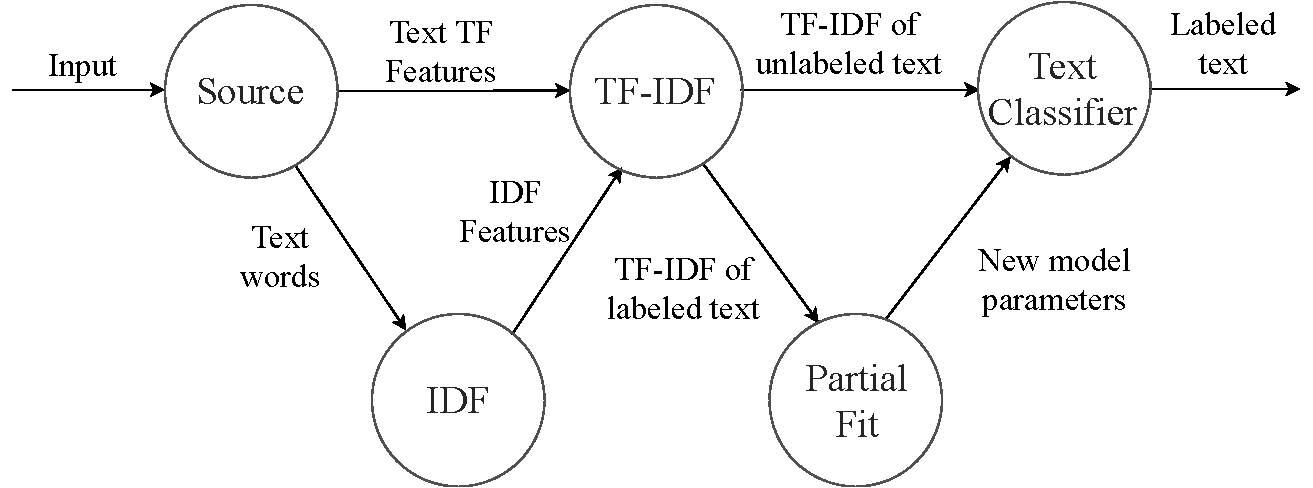
\includegraphics[scale=0.48]{pics/logical-graph}
  \caption{The logical pipeline}
  \label {logical_graph}
\end{figure}

For our task, the calculations can be illustrated as a logical graph illustrated in Figure~\ref{logical_graph}. Input vertex receives incoming texts, calculates term frequencies and transfers them to the TF-IDF vertex. It also sends words from the text to IDF vertex. IDF computes the inverse frequency of the words and delivers them to the TF-IDF vertex. TF-IDF joins corresponding inverse documents frequencies together with term frequencies within a given text. After that, the complete TF-IDF features are sent to Text Classifier vertex. Classifier predicts the label and delivers the result to the user.

\begin{figure}[htbp]
  \centering
  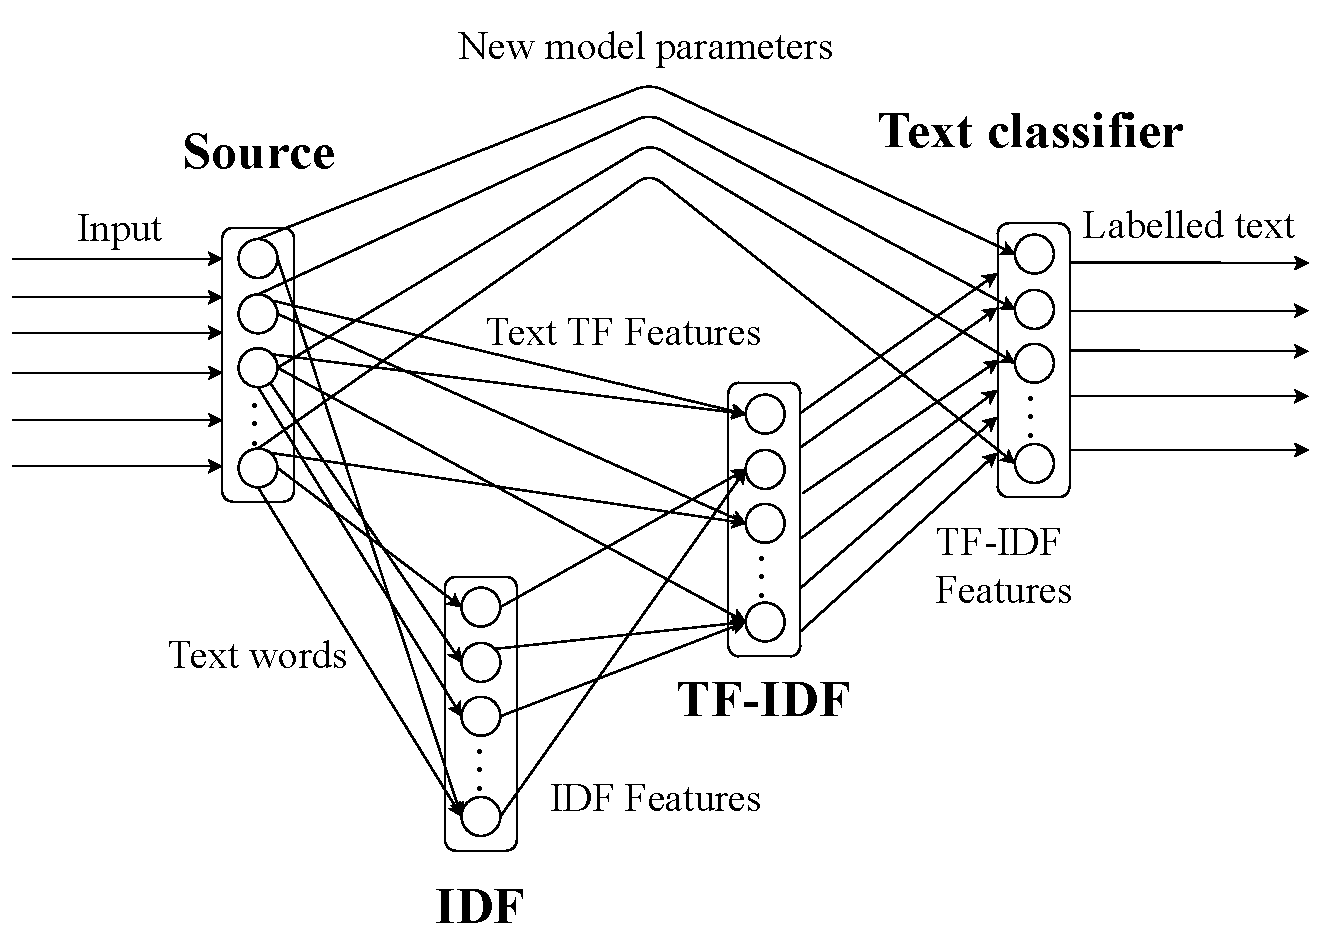
\includegraphics[scale=0.375]{pics/physical-graph}
  \caption{The physical pipeline}
  \label {physical_graph}
\end{figure}

When the pipeline is deployed, the logical graph maps into a physical graph(Figure ~\ref{physical_graph}). Each logical task is mapped to a number of physical tasks. This is, every vertex here is a single computational unit. Each rectangle denotes the same cluster of computers.

Input texts are received by all machines. Shuffle before IDF vertex are defined by a hash function of a word. Partitioning before TF-IDF physical vertices are determined by a text id. There is no network shuffle between TF-IDF and Text Classifier vertices, so they are simply chained. The partial Fit operation is located on a single machine and broadcasts model parameters to Classifier vertices.

%That is, real calculations are defined by the physical graph and can be described as follows. Input text can be received by any machine. Then Text Document vertex produces a list of words for the text and the list is distributed among all shards using the described scheme. In case of words with a high frequency such as conjunctions or prepositions, we add to them salt to the end thereby spreading all the words between the shards evenly. After that, a list of words distributed among all shards for IDF processing using the technique. In the TF-IDF stage, IDF features of the same document accumulate on a particular shard using the scheme. In the IDF and TF-IDF stages the same sharding method is used, however, the difference is during IDF processing sharding is done by a word and during TF-IDF -- by a text document. Accumulated IDF features join with the corresponding TF features. In the Text Classifier stage, classifier obtains a label for the text and returns it to the user. During this stage, the classifying process is done on the same machine, where TF-IDF features were gathered together.

\subsubsection{Dealing with concept drift}

Concept drift is a phenomenon of changing users' interests from time to time, which usually depends on recent events, and results in shifting the distribution of text classes to particular ones. Essentially, this may affect the correctness of the pipeline, more specifically, the computing of the IDF features. To overcome the issue, we use windowed IDF calculation: concrete IDF values will be provided based on input within a time window. For instance, the window can be set to a day or a week. This scheme allows us to deal with sudden changes in the topics. Similar approaches are applied in [?].

\subsubsection{Partial fit}

Figures ~\ref{logical_graph}, ~\ref{physical_graph} provide a scheme for a partial fitting. Labeled input documents accumulate in the Partial Fit vertex. Additional training is triggered by a special element, which is submitted to the input as an ordinary element. However, this element is not processed as a text and the vertices just push the element further. This process is similar to punctuation processing \cite{tucker2003exploiting}. The conditions, when the partial fitting starts, can be chosen arbitrarily by a system administrator. For example, one can update machine learning model on every 1000 labeled documents.

\subsection{ML model \label{ML}}

The classifier's model can be chosen independently from other computations. In our case, we use Multinomial Logistic Regression. At the start of the system, the initial classifier parameters such as weights can be provided by a pre-train process.

Every time, when the Partial Fit is triggered, the following process occurs, which can be described in terms of the optimization of a cost function. This function in our case is written below:

\begin{center}

$$ J(W) = -\frac{1}{m} \sum \limits_{i = 1}^{m} \sum \limits_{j = 1}^{k} \mathbbm{1}_{\left\{y^{(i)} == j\right\}} \cdot \log \frac{\exp\left({W_{j}^Tx^{(i)}}\right) }{\sum \limits_{l = 1}^{k}  \exp\left({W_{l}^Tx^{(i)}}\right) }$$ 
 $$ +  \lambda_1 ||W||_1 + \lambda_2 ||W - W_{prev}||_2 $$

\end{center} 

The number of points in a new dataset is denoted as $m$. The point with index $i$ showed as $x^{(i)}$. The number of classes is $k$. New weights are designated as $W$. The weights, that computed in the previous step, are $W_{prev}$. At the first time of triggering the process, $W_{prev}$ are the pre-trained weights. 

The formula provides the goal of the training. The first component is the standard softmax function for multiple classes. The second component keeps the l1 regularization of the weights. The important aspect is the regularization provides sparsity, hence, the model has a small size -- about 15 Mb, which can be stored and updated with low cost. To use the previous history of the classifier weights we apply l2 regularization as the third component. Fitting new points and the consideration of the previous weights ensure better accuracy of the classifier.

We are interested in finding such $W$ that minimizes $J(W)$. Taking derivatives, one can show that the gradient for each class component is:

\begin{center}

$$ \nabla_{W_j} \; J(W) = -\frac{1}{m} \sum \limits_{i = 1}^{m} \left[ x^{(i)} \left( \mathbbm{1}_{\left\{y^{(i)} == j\right\} } - \frac{\exp\left({W_{j}^Tx^{(i)}}\right)}{\sum \limits_{l = 1}^{k}  \exp\left({W_{l}^Tx^{(i)}}\right)} \right) \right] $$
$$ - \; \lambda_1 sign\left(W\right) - \frac{\lambda_2}{2} \left(W - W_{prev} \right), \; j = [1..k] $$

\end{center} 

We use Stochastic Gradient Descent for optimization. In experiments ~\ref{fs-short-experiments} section, model performance is presented.

\section {Evaluation}
\label {fs-discussion}

In this section, we discuss and demonstrate the main pitfalls which arise with the na\"ive data flow. The purpose of our evaluation is to investigate the applicability of stream processing systems as a {\em tool} for building text classification pipelines rather than to compare various machine learning models. We concentrate on a question on how distributed stream processing features may affect reproducibility and reliability of classification results.

For experiments, we used an implementation of the proposed data flow on top of Apache Flink~\cite{Carbone:2017:SMA:3137765.3137777}. Apache Flink is a state-of-the-art industrial stream processing engine that is one of the most performant among competitors~\cite{karimov2018benchmarking, S7530084}. The experiments were performed on a single 4 core CPU 8GB RAM machine with 2 Flink workers. Such setting is chosen to show that issues can be faced even in a deployment with a limited asynchrony. As a dataset, we used an open corpus of news articles from Russian media resource lenta.ru~\cite{lentaru}. This dataset contains documents, which are labeled by one of 90 different topics such as {\em sport}, {\em politics}, {\em science}, etc. For the experiments, we generated a stream consisted of articles from the dataset. Processing {\em latency} in such setting is a time period between article arrives at the system entry and a corresponding label given by a classifier is released. 

We used multinomial logistic regression model as a classifier. We mainly considered the multi-classification problem, but also saw into the label probability distribution obtained by an article. For instance, text about novel research in sports food may be denoted as 70\% about sport, 20\% about science and 10\% about food. In this case, it may be reasonable to take into consideration the top $n$ most probable labels rather than only the winner topic (sport).

\subsection{Reproducibility}

Users of popular open-source machine learning libraries like sklearn~\cite{sklearn_api} used to obtain results which are unbiased by an execution environment. Migration to batch processing systems like Hadoop~\cite{hadoop2009hadoop} or Spark~\cite{Zaharia:2016:ASU:3013530.2934664} usually do not cause many extra issues, because these engines mostly hide effects of asynchronous processing from a user and provide deterministic results. On the contrary, most distributed stream processing engines are non-deterministic due to processing model aiming to low latency. Therefore, the main challenge regarding reproducibility of streaming machine learning pipelines is to achieve predictable results, while keeping low processing latency.

\subsubsection{Races in the data flow}
The issue is that there is a race between documents in the data flow before IDF update. Hence, IDF features of the words in articles may vary from run to run. For example, let us consider two documents stream: the first one contains word {\em cat}, while the second consists of {\em cat} and {\em dog}. If the first document is processed before the second, IDF for the word {\em cat} within TF-IDF features of the second document will be 1, while otherwise, it will be 0.

To show how this behavior affects text classification results we made 10 runs on a stream consisted of 10 000 news articles. We compared the most probable 1,2,3,4,5 obtained labels for the same documents between runs. Our comparison was order-sensitive: if top 2 labels for the document on the first run is [sport (50\%), science (20\%)], but on the second run [science (50\%), sport (20\%)], then we denoted these results as varied. 

Table~\ref{race_table} demonstrates the results of the experiment. As we can see, approximately 56 out of 10 000 articles obtained different the most probable label. With the growth of the number of the labels that we consider, the percent of varied results significantly increases: 1270 articles achieved different top 5 labels on the average. These results indicate that the issue may influence the classification results and makes them hardly reproducible between independent runs. Another negative effect of non-deterministic data flow is an increase in results variance. It may be unclear which reason causes accuracy changes: modification of the model or just another order of IDF updates.

\begin{table}[htbp]
\caption{Effects of races in the data flow}
\begin{threeparttable}
\begin{tabular}{lcl}
Top labels for comparison    & \% of varied results & std    \\
\hline
1   &   0.56    &   0.06    \\
2   &   2.38    &   0.14    \\
3   &   5.27    &   0.22    \\
4   &   9.27    &   0.35    \\
5   &   13.7    &   0.53    \\
\end{tabular}
\end{threeparttable}
\label{race_table}
\end{table}

\subsubsection{Overhead on enforcing reproducibility}

A straightforward technique to avoid races before IDF update is to define a synthetic total order on input documents and to enforce such order before the operation that modifies IDF. In Flink, the order can be defined using timestamps assigned to input elements. Order enforcement is implemented using custom {\it ProcessFunction} that buffers all words before IDF update. In order to flush this buffer, there is a need to ensure that all words from the document with a particular timestamp have arrived. Such guarantee can be provided by {\em low watermarks} mechanism. Low watermarks are service stream elements which go through the same network channels as ordinary elements and guarantee that there are no items with a given or less timestamp up to the stream. Hence, we can flush parts of the buffer when a corresponding watermark arrives. Such implementation follows {\em out-of-order} processing approach~\cite{Li:2008:OPN:1453856.1453890}.

Figure~\ref{reproducibility} demonstrates the comparison in latency between reproducible and irreproducible data flows. We compare $50^{th}$, $75^{th}$, $95^{th}$, and $99^{th}$ percentile of distributions, which clearly represent the performance from the perspective of the users' experience. Latency overhead is 50\% (11 ms) for the median and 24\% (28 ms) for the 99th percentile. This behavior indicates that the overhead is moderate in a general case. However, it may be sensitive for applications with extremely low latency requirements.

\begin{figure}[htbp]
  \centering
  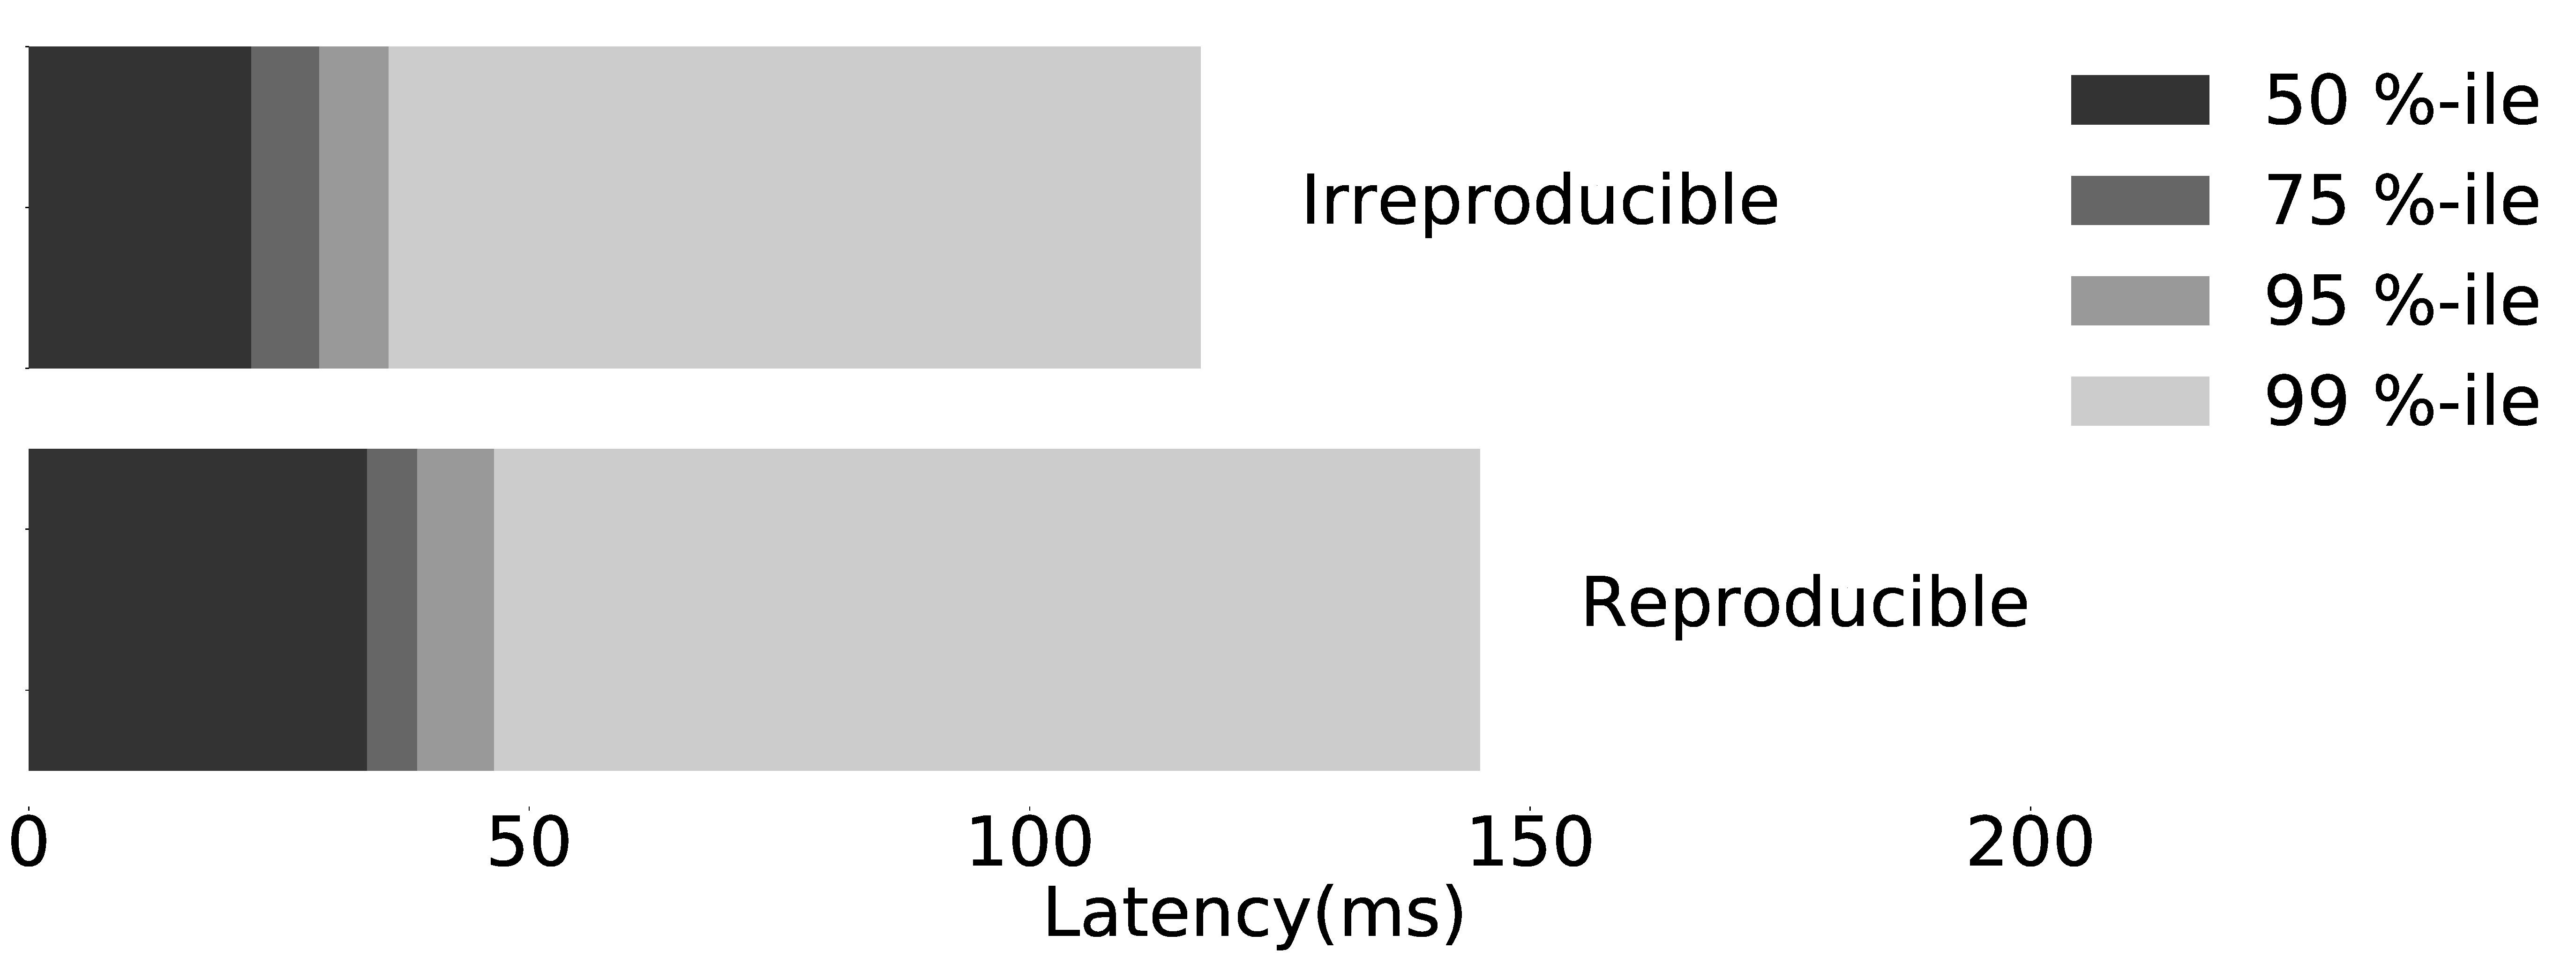
\includegraphics[scale=0.09]{pics/reproducibility}
  \caption{Latency comparison between reproducible and irreproducible data flows}
  \label {reproducibility}
\end{figure}

\subsection{Fault tolerance}

As we demonstrated above, if machine learning pipeline runs on multiple computational units, there can be issues with reproducibility. Unfortunately, it is not the only challenge: computational nodes and network failures may potentially cause shifted or even incorrect results. Despite the fact that failures are typically considered as edge cases, incorrect results obtained due to even rare instabilities may affect service reputation and lead to financial losses. Hence, in large-scale production deployments, it is important to ensure that nodes and network failures do not influence the outcome.

In stream processing systems, guarantees on data in case of failure are typically described in terms of {\em delivery guarantees}: at least once and exactly once. If a system provides exactly once, it is guaranteed that a streaming element is applied to data flow operators and released exactly one time. In other words, a system ensures that failure would be transparent for end-user. With at least once, it is ensured that an element is not lost, but it can influence operator states and be delivered to end-user multiple times. At least once may be preferred, because it typically has lower performance overhead. However, it is unclear in what degree such relaxation can influence the classification results. 

In order to demonstrate how the choice of a delivery guarantee affects text classification pipeline, we model two scenarios that can be faced, e.g. in news aggregators:
\begin{enumerate}
    \item There are two equally important events at the same time, e.g. football world cup and the G20 summit. Arriving news stories are grouped by these events: $n$ texts about football, then $n$ texts about politics and so on. This arrangement simulates articles from multiple sources. We expect that the proportion between the number of texts labeled as football and number of texts labeled as politics would be similar to the real distribution. Otherwise, news aggregator can make wrong conclusions about event importance and impact. The arose question is: can failure within at least once guarantee bias such distribution?
    \item Assume that news aggregator denotes topic as {\em popular} if the percent of articles labeled by this topic exceeds some threshold. For instance, in a day of Olympics opening ceremony, we expect that topic {\em sport} becomes popular as well as usual prevalent themes like politics or business. We simulate such a situation when some theme overcomes a given threshold under a normal execution or exactly once guarantee. Within the confines of this experiment, we aim to study if a failure under at least once guarantee can cause that the event does not exceed the threshold.    
\end{enumerate}

% In the following experiments, we demonstrate that at least once guarantee may not be acceptable in some cases. 

For the experiments, we set up 1 second between checkpoints in Flink, {\em RocksDB} as a state backend, and at least once as a delivery guarantee. It is worth to note that 1 second is the minimal snapshotting period that we were able to reproduce. The larger period can imply even more significant effects because in this case more elements are processed more than one time if a failure occurs.

\subsubsection{Biased results distribution}

In this experiment, we used a stream with 4000 articles. These articles can be considered as stories within a fixed time window and we are interested in the news topics distribution in this window. Articles are grouped in 4 blocks: 1st and 3rd contain news about football, and 2nd and 4th consisted of science news stories. We simulated a single node failure in both football and science groups. We denote that an article is classified into topic {\em Z} if it has the largest probability among all topics. Results are shown in Table~\ref{biased_results}. As one can notice, the classifier has an error: it labels approximately 42\% of articles as football and 40\% as science stories, while others are mistakenly classified as other topics. Nevertheless, it is important that results indicate a small difference between the number of football and news articles - about 1.5\%. The failure causes a significant shift of this distribution: as expected, a failure during football or science news implies repeated processing of the same articles. In both cases, there were repeated about 600 texts. As a result, we can see that the biased distribution, that is hardly similar to the original: the difference between the number of articles labeled as football and science becomes 7-10\%. 

\begin{table}[htbp]
\caption{Biased classification results due to failure within at least once guarantee}
\begin{threeparttable}
\begin{tabular}{lcl}
Experiment    & \% of football articles & \% of science articles    \\
\hline
Ground truth   &   50.0    &   50.0    \\
No failures*   &   41.8    &   40.4    \\
Failure on football**   &   46.7    &   35.5    \\
Failure on science**   &   37.7    &   44.5    \\
\end{tabular}
* or with enabled exactly-once \\
** with enabled at least once
\end{threeparttable}
\label{biased_results}
\end{table}

\subsubsection{Invalid threshold}

% In the previous experiment, we demonstrated that failures can noticeably influence the distribution of classification results if there are few topics in an input stream. In this one, we show that the problem exists in a more general case. 

Test stream for this experiment contains 5000 articles. As in the previous experiment, we can denote them as news stories within a fixed time window. First 4450 articles in a stream have all possible 90 topics with the prevalence of football and politics. Last 550 texts consisted of news about animals. Such setup simulates some emerging event connected to animals. Assume that a news aggregator denotes topic as popular if it exceeds threshold 10\%. We simulated a single failure when the first 4450 articles were being processed.

Results of the experiments are shown in Table~\ref{biased_threshold}. It is expected that topic {\em animals} becomes popular. Without failures, this assumption is satisfied. However, failure with reprocessing of approximately 600 articles shifts the distribution of topics in results: the percent of articles labeled as animals story becomes 0.094. In this case, is not considered as popular and such behavior may affect news aggregation business logic.

\begin{table}[htbp]
\caption{Biased threshold due to failure within at least once guarantee}
\begin{threeparttable}
\begin{tabular}{lcl}
Experiment    & Top 3 topics    \\
\hline
Ground truth   &   Politics(11.5), Football(11.3),Animals(11.0)    \\
No failures*   &   Football(10.7),Animals(10.1),Politics(10.0)    \\
Failure**   &   Football(10.8),Politics(10.3),Animals({\bf 9.4})    \\
\end{tabular}
* or with enabled exactly-once \\
** with enabled at least once
\end{threeparttable}
\label{biased_threshold}
\end{table}

\subsubsection{Overhead on exactly once}

In order to avoid results inconsistencies in case of failures, there is a need to enable exactly once delivery guarantee. Exactly once is implemented in Flink using a modification of the 2PC transactional protocol. A transaction starts when Flink injects a special element called {\em checkpoint} into the input stream. Each operation independently prepares data to save at the moment of checkpoint arrival. Prepared data is committed to external storage when checkpoint passes through the whole data flow. Output elements are released only after the transaction is committed. Because of the fact that a transaction begins once per snapshotting period, this period directly influences the latency of individual streaming elements.

Figure~\ref{fault_tolerance} shows latency comparison between runs within at least once and exactly once guarantees in Flink. As expected, latency in exactly once mode depends on the snapshotting period. Overhead on latency is significant even with 1 second between checkpoints: it is more than a second for all considered percentiles. Such behavior can be unacceptable in many real-life applications. Hence, there is a trade-off between latency of individual elements and a guarantee that failures do not affect classification results.

\begin{figure}[htbp]
  \centering
  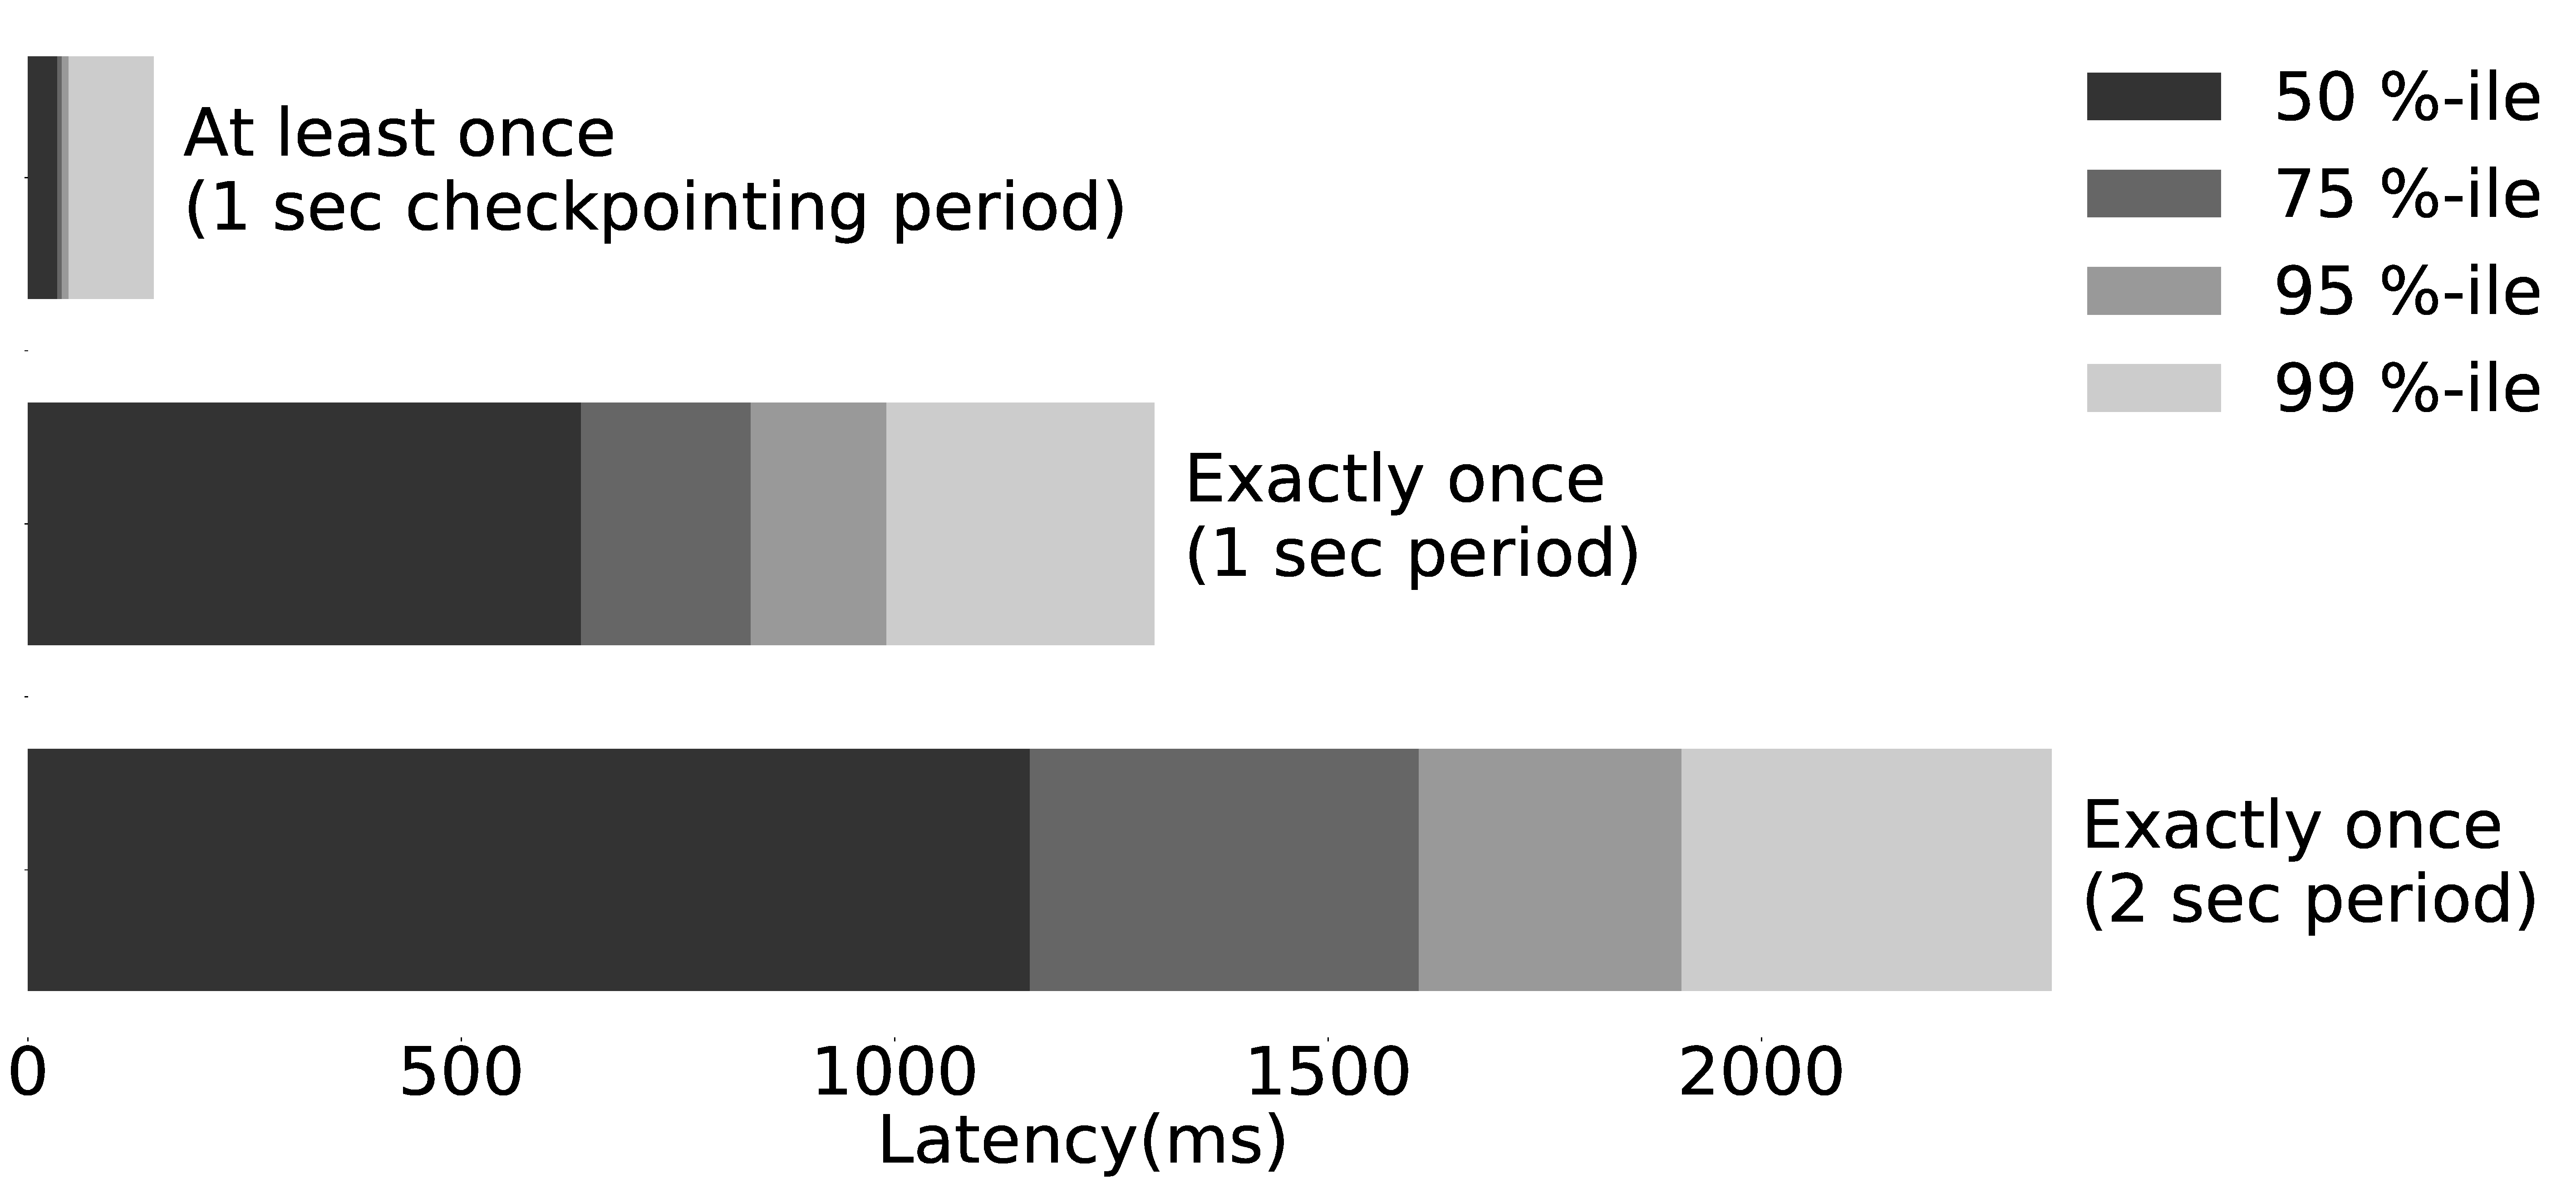
\includegraphics[scale=0.09]{pics/fault_tolerance}
  \caption{Latency overhead on exactly once}
  \label {fault_tolerance}
\end{figure}



\section {Screaming challenges}
\label {fs-solution}

\subsection{Reproducibility and Fault Tolerance}

{\em Exactly-once} and determinism are desirable properties for the text classification data flow. On the other hand, one of the key performance metrics in streaming applications is latency. Table~\ref{comparison} shows if a system supports exactly-once, built-in determinism, and low latency (less than 500 ms). To the best of our knowledge, among open systems only~\FlameStream\ provides for both low latency, determinism, and exactly-once. This property is achieved using optimistic total order enforcement. The details of this approach are discussed in~\cite{we2018adbis, we2018beyondmr}. Implementation of the text classification data flow on top of~\FlameStream\ can potentially resolve the trade-offs between reliability and performance.

\begin{table}[htbp]
\caption{Comparison of stream processing systems}
\begin{threeparttable}
\begin{tabular}{lccc}
System & Exactly-once & Determinism & Latency    \\
\hline
Storm, Heron, Samza  &    --      &   --       &   low            \\
Spark Streaming    &    +       &   +        &   high           \\
Flink              &    +       &   -        &   high$^*$       \\
MillWheel          &    +       &   +        &   NA             \\
FlameStream        &    +       &   +        &   low            \\
\end{tabular}
* with enabled {\em exactly-once}~\cite{we2018beyondmr}
\end{threeparttable}
\label{comparison}
\end{table}

\subsection{Concept Drift}

Streaming applications often experience {\em concept drift}: the statistical properties of the target, which the machine learning model is trying to predict, change over time. Regarding news articles classification, concept drift may lead to the following effects:

\begin{itemize}
    \item Meaning of some terms is changing over time. For example, word {\em goal} in the article published during the soccer world cup is most likely related to soccer. On the other hand, during the world hockey cup, it rather belongs to the hockey topic.
    \item News topic may appear and vanish over time. For example, some important events can transform into a separate news topic for a time as it happens with large political or sports forums. However, after some time such topics can disappear form a news agenda.
\end{itemize}

A streaming classifier must handle such behavior to automatically fit in rapidly changing news data. We propose a modification of the data flow for prediction with online training that aims to handle concept drift. Training is a separate branch within the logical graph presented in section~\ref{fs-framework}. The modified data flow is shown in Figure~\ref{training_graph}. Assume that the input stream consists of two types of elements: pre-labeled and raw. The latter elements must be labeled by a classifier and delivered to end-user. For already labeled text its features are sent to a {\em Partial fit} vertex instead of the {\em Classifier}. {\em Partial fit} vertex updates machine learning model and sends it to {\em Text Classifier} vertice.

\begin{figure}[htbp]
  \centering
  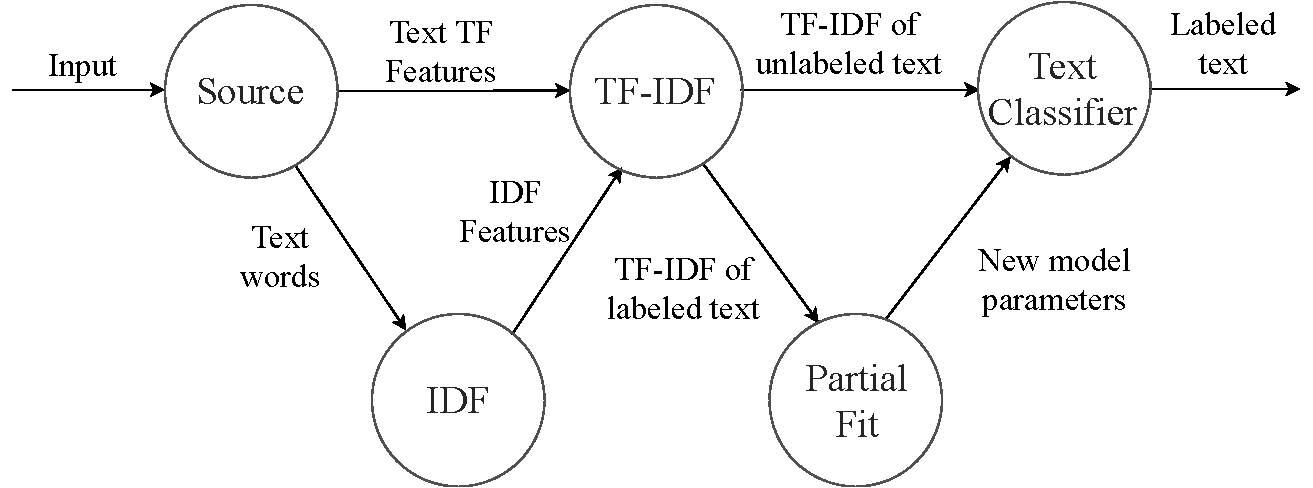
\includegraphics[scale=0.32]{pics/logical-graph}
  \caption{Data flow with online training}
  \label {training_graph}
\end{figure}

A potential issue is that the training process may be time-consuming. If training and prediction processes run consecutively, there will be significant latency spikes, e.g. if a training process lasts for several minutes, then spikes can be thousands times greater than the latency for prediction. However, without synchronization, there will be no reproducible correspondence between texts and applied model. It is almost impossible to achieve the same results within a new run on the same data because the training time becomes a hidden parameter that influences output. 

For instance, assume that we make two runs. On the first run model update takes 70 seconds, but on the second run 75 seconds due to extra CPU load. If training and predicting are not synchronized, more unlabeled input elements are processed by an outdated model in the second case so the distribution of news topics may be different between these two runs. To solve this issue, we propose using efficient online learning algorithms, e.g. FTRL proximal~\cite{mcmahan2013ad}. In this case, model updating is smooth and its synchronization with training does not cause latency spikes.

\section{Related Work}


Most related prior works were implemented on Apache Spark \cite{semberecki2016distributed} \cite{8029336} \cite{Nodarakis2016LargeSS} \cite{baltas2016apache} \cite{svyatkovskiy2016large} or Apache Storm \cite{khumoyun2016real}. These platforms use micro-batching technique for processing data. However, such method provides high latency between obtaining a text and labelling it. In addition, all the methods above does not consider a concept drift as an issue.

Next work takes into account the concept drift and related to stream data nature \cite{zhang2008one}. However, the final solution is hard to scale into a cluster of machines efficiently.

\section {Conclusion}
\label {fs-conclusion}

In this work, we investigated the suitability of distributed stream processing engines to the problem of text streams classification. We demonstrated that there are several pitfalls with an adaptation of data flow commonly used in batch systems for a stream processing:

\begin{itemize}
    \item Races in a physical data flow lead to irreproducible results: labels provided by a classifier may vary from run to run on the same test data. 
    \item Failures within {\em at least once} delivery guarantee can cause a biased distribution of classification results.
    \item Streaming data is rapidly changing, so there is a need to update the machine learning model on-the-fly. 
\end{itemize}

It was shown that straightforward solutions to the mentioned issues imply significant performance overhead. There were proposed potential solutions: to use~\FlameStream\ processing system with built-in determinism and efficient exactly once and to embed online learning into the data flow. 

As future work, we plan to implement a text classification framework that satisfies the following requirements:

\begin{itemize}
    \item Unbiased by distributed environment: node failures or races do not affect the ultimate result distribution.
    \item Reproducible: if input elements are stored in persistent storage, the same predictions are obtained on each new run.
    \item Concept drift conscious: changes in streaming data must be reflected in a machine learning model.  
\end{itemize}

\bibliographystyle{ACM-Reference-Format}
\bibliography{../../bibliography/flame-stream}

\end {document}

\endinput
